\section{Results I: Learnable Chain-Coupling, Verifier Accuracy and Generalization}
\label{sec:results_main}

This section reports the central empirical claim of the system: that a genuine
Truth Beam recording contains a learnable physical coupling between the captured
raw frame $C_t$ and the chain-derived emission $E_t$, and that this coupling is
strong enough to support a near-perfect verifier on held-out data. We present
the headline verifier accuracy, the control experiment that isolates the
coupling signal from generic emission statistics and architecture artifacts, the
frame-level operating-point analysis on the full corpus, and the same-rig
cross-session and cross-protocol generalization result. We are deliberate about
scope: every quantitative claim below is a \emph{same-rig} result over two
recording sessions (D2 and V10) of a single performer, and the only trained
adversary exercised is F-A~v1. We make no cross-rig,
cross-camera, cross-projector, or cross-subject claim, and no claim of
robustness against a stronger adaptive attacker; those limits are restated
explicitly at the points where they bind. Throughout, held-out evaluation
scores a fixed subsample of the held-out blocks: $n=198$ frames for D2
(66 from each of its three blocks) and $n=200$ for V10 (100 from each of
its two blocks).

\subsection{Headline verifier accuracy}
\label{sec:results_main_headline}

The load-bearing verifier is the Phase~G diffusion model (\Cref{sec:verifier_method}):
a custom \num{39.77}M-parameter $\epsilon$-prediction U-Net with ControlNet-style
emission conditioning, operating frame-by-frame on a single $(C_t, E_t)$ pair.
It never denoises; it scores a capture by the noise-prediction residual
$\lVert \hat{\epsilon}-\epsilon\rVert^2$, averaged over five fixed evaluation
timesteps $\{50,150,300,500,750\}$ and $K_{\text{NOISE}}=4$ noise samples per
$(C,E,t)$. A capture that is consistent with its recorded chain-coupled emission
yields a low residual; a capture paired with the wrong, shuffled, or synthetic
emission yields a higher residual.

On held-out evaluation blocks the verifier separates the correct emission $E_t$
from temporally mispaired (offset) wrong emissions perfectly:
\textbf{AUROC = 1.000} on both the D2 held-out set ($n=198$) and the V10 held-out
set ($n=200$). The separation is large and tightly bounded. On D2 the mean
$\epsilon$-residual is $0.00348$ for the correct emission versus $0.00748$ for
the average wrong emission, a gap of $\Delta_{\text{wrong}} = +0.00400$
(\SI{95}{\percent} CI $[+0.00397, +0.00403]$). On V10 the corresponding values
are $0.00394$ versus $0.00804$, a gap of $\Delta_{\text{wrong}} = +0.00411$
(\SI{95}{\percent} CI $[+0.00410, +0.00411]$). These are finite-sample point
estimates: at $n \approx 200$ a measured AUROC of $1.000$ is consistent with a
true pairwise error rate up to roughly the one-percent scale, and we
deliberately do not attach asymptotic confidence intervals to a
perfect-separation estimate; the claim is exact separation \emph{on these
evaluation sets}, no more. The lag sweep over chain
alignment confirms that the residual minimum sits at the correct alignment: on
D2 the lag-0 residual is $0.003484$ against $0.007488$ at lag $-1$ and $0.007487$
at lag $+1$; on V10 the lag-0 residual is $0.003938$ against neighbours near
$0.00804$. Every offset lag sits on the high wrong-$E$ plateau, so the correct
emission is not merely best on average but is sharply distinguished from its
immediate temporal neighbours.

The discriminative signal is strongest at small diffusion timesteps and decays
as $t$ rises, consistent with the coupling living in the higher-frequency
structure of the capture that low-noise reconstruction is most sensitive to. The
per-timestep AUROC is $1.000$ at every reported primary timestep, while
$\Delta_{\text{wrong}}$ falls monotonically: on D2 it is roughly $0.00594$ at
$t=150$, $0.00339$ at $t=300$, and $0.00165$ at $t=500$ (V10 behaves
near-identically). The verifier is therefore not relying on a single timestep;
it accumulates a graded, schedule-wide signal.

\subsection{The coupling signal is real, not an emission-statistics or architecture artifact}
\label{sec:results_main_control}

A perfect AUROC invites the obvious skepticism: perhaps the verifier merely
detects that \emph{some} emission is present, or exploits an architectural
shortcut, rather than learning the genuine $C_t$--$E_t$ coupling. We rule this
out with an architecture- and data-matched \emph{shuffled control}. The control
is identical to the main verifier in every respect --- same backbone, same
parameter count, same training data, same training budget --- and differs only
in the real-versus-shuffled pairing of $C$ and $E$ during training. If the
network could discriminate from generic emission statistics or from any property
of the architecture, the shuffled control would also separate correct from wrong
emissions. It does not: the shuffled control sits at chance, with
\textbf{AUROC $\approx 0.5006$} (D2 $0.5006377$, V10 $0.500625$), and its
correct-versus-wrong residual gap collapses to
$\Delta_{\text{wrong}} \approx 10^{-7}$ (D2 $6.98\times10^{-8}$, V10
$1.39\times10^{-7}$, \SI{95}{\percent} CI $[1.07\times10^{-7}, 1.71\times10^{-7}]$).
Although the control's \SI{95}{\percent} CI for $\Delta_{\text{wrong}}$ technically
excludes zero, the effect is roughly five orders of magnitude smaller than the
main run's $\Delta_{\text{wrong}} \approx 4\times10^{-3}$ --- operationally
indistinguishable from chance. The contrast between AUROC = 1.000 (main) and
AUROC $\approx 0.5006$ (shuffled control) is the cleanest evidence we have that
the verifier's accuracy derives from the genuine physical chain-coupling between
capture and emission, not from an emission-statistics or architecture shortcut.

A complementary synthetic-positive control confirms the converse: that the
evaluation pipeline \emph{can} detect an emission-dependent signal when one is
deliberately injected. Adding an isotropic photometric injection (a blurred
emission added back into the capture) produces AUROC = 1.000 on both sessions
with a measurable residual gap ($\Delta_{\text{wrong}} = +0.00113$ on D2,
$+0.00122$ on V10). This establishes that a null result in the shuffled control
reflects the absence of a coupling signal in shuffled pairs rather than a dead
pipeline. We note the limitation that the synthetic injection is isotropic,
whereas the real chain signal may have different spectral structure, so the
synthetic pass alone does not certify the main pass; it is corroborative, not
load-bearing.

\subsection{Frame-level separability on the full corpus}
\label{sec:results_main_framelevel}

The held-out blocks above are the model's own verifier-tier evaluation. To
characterize separability over the entire dataset under a calibrated display
recipe, we additionally report frame-level metrics from the substrate-verification
visualization run, scored over the full \num{9735}-frame corpus (D2 + V10) at the
Phase~G K2 robust-$z$ residual. Each frame contributes a single observation whose
score is the mean per-pixel $z_{\text{two}}$ residual. At the frame level the
verifier achieves \textbf{AUROC = 0.9999} separating real-correct captures from
real-shuffled-$E$ captures, and \textbf{AUROC = 0.9998} separating real-correct
captures from synthetic (F-A~v1 fake) captures at adversary training step
\num{100000}. \Cref{fig:roc} shows the corresponding ROC curves alongside the
per-frame mean-$z_{\text{two}}$ distributions. The mean per-frame
$z_{\text{two}}$ is $1.06$ for real-correct captures, $4.19$ for shuffled-$E$,
and $3.59$ for the step-\num{100000} fake; the real-correct mode is well separated
from both anomalous modes.

These frame-level AUROCs are distinct from, and should not be conflated with, the
Phase~G model's own training-tier AUROC of $1.000$: they are computed at the
frame level under a fixed calibrated recipe over the whole corpus, and they
measure rank-order separability between conditions on the evaluated frame set
rather than a deployed fixed-threshold operating point. A precision note for
re-computation: the released compact per-frame table
(\texttt{visual\_metrics\_wide.csv}, \Cref{sec:availability:derived}) reproduces
these contrasts at $0.9998$ for both (and mean per-frame $z_{\text{two}}$ of
$1.07/4.10/3.54$); the $0.9999$ figure and the $1.06/4.19/3.59$ means quoted
here and in the figures are the visualization run's own aggregate over the
full-resolution maps, which the compact table summarizes slightly differently
--- the difference is one unit in the fourth decimal and does not affect any
conclusion. We also stress that the
$0.9999$/$0.9998$ figures are \emph{pooled} frame-level numbers; the per-pixel
AUROC is substantially lower (mean $0.74$, max $0.99$), and pooling across pixels
is what reaches near-unity. The headline numbers are not per-pixel claims.

\Cref{fig:zhist} and \Cref{fig:ecdf} (\Cref{sec:verifier_method}) make the
distributional basis of this separability explicit: the real-correct
$z_{\text{two}}$ mass concentrates at low $z$ (the real-correct empirical CDF
reaches $0.95$ at $z=3.0$), while shuffled and synthetic conditions carry heavy
right tails that only reach the same percentile at substantially higher $z$. The
discriminative substrate signal is precisely this rightward-shifted tail above
the high percentiles of the per-session reference. Under the calibrated recommended
display recipe, real-correct frames render essentially uniformly green --- mean
red area $0.018\%$ --- while shuffled and synthetic frames are heavily red on the
excess panel, at $53.2\%$ (shuffled) and $51.4\%$ (synthetic) mean red area over
the full corpus. \Cref{fig:hero} shows this contrast across fourteen
representative captures, and \Cref{fig:main_results} assembles the composite
result, the attacker-maturity progression, the $z_{\text{two}}$ densities, and
the ROC into a single figure.

\begin{figure}[tp]
\centering
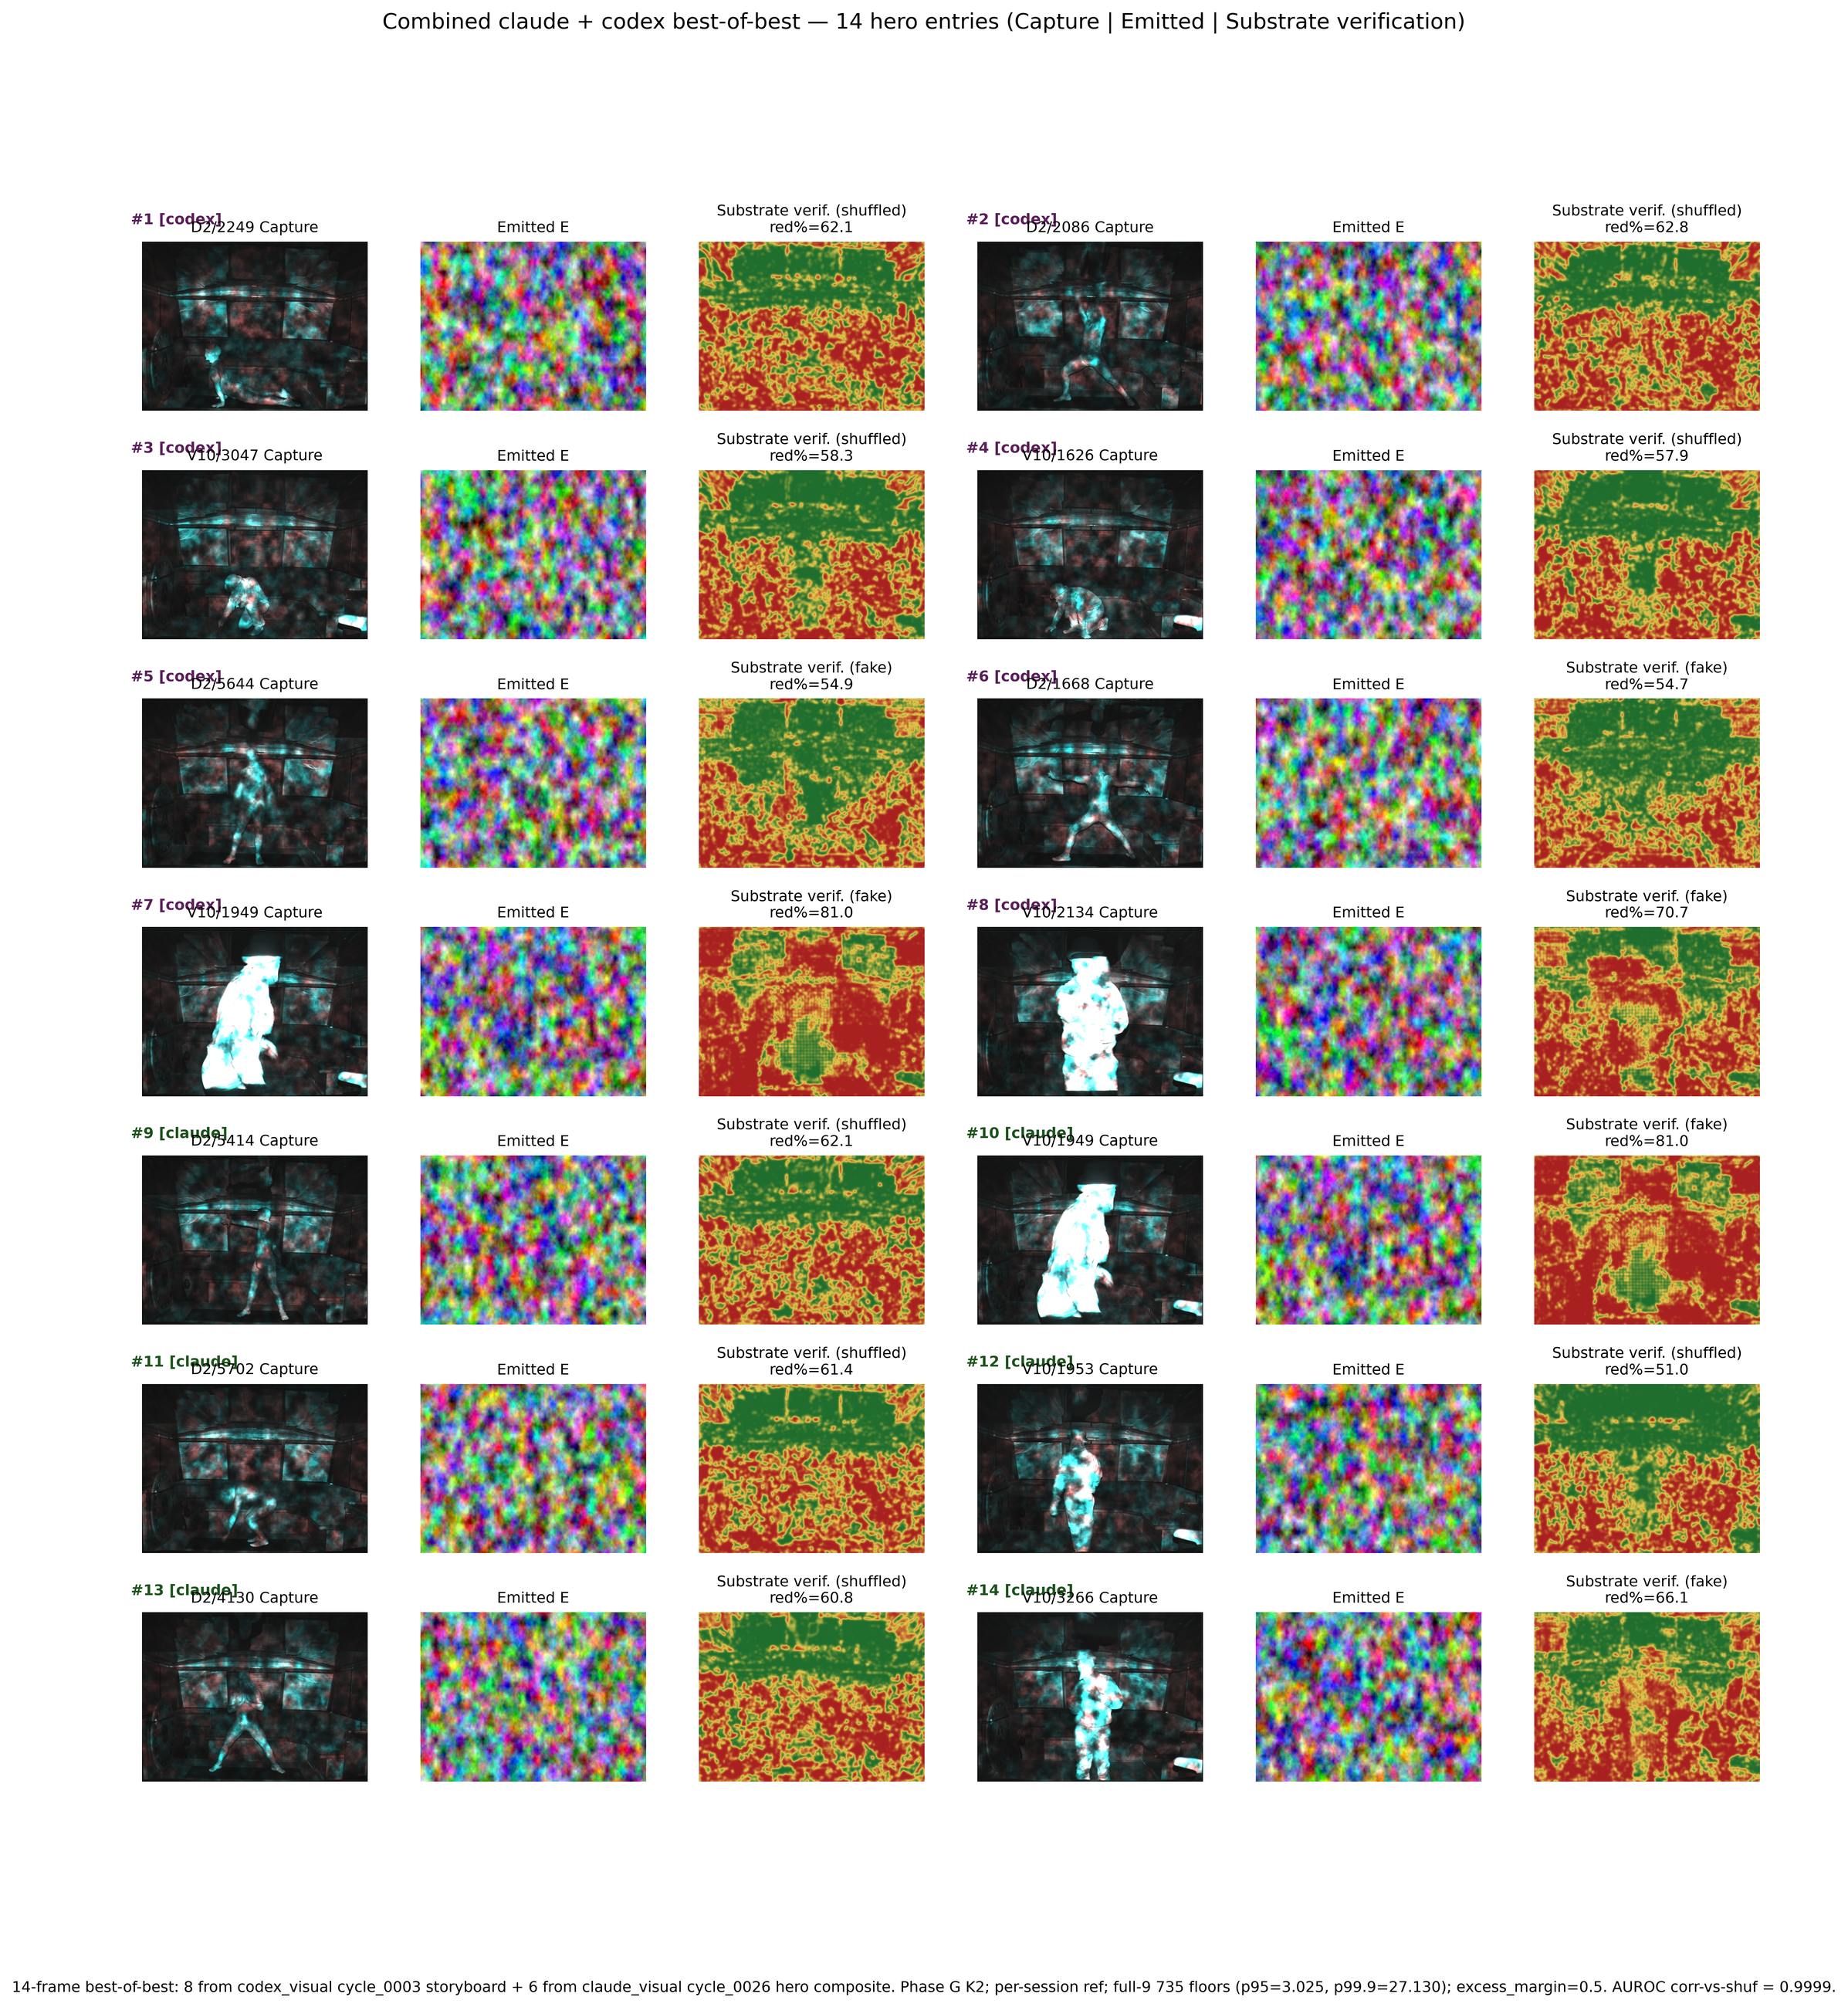
\includegraphics[width=\linewidth]{figures/fig_hero.png}
\caption{Substrate verification at a glance. Fourteen representative captures,
each shown as raw camera frame $C$, the emitted chain-coupled pattern $E$, and
the per-pixel substrate-verification map (Phase~G robust $z$-residual;
green~$=$~typical of a genuine chain-coupled capture, red~$=$~anomalous).
Real-correct frames render essentially uniformly green; substrate-altered
conditions (shuffled or synthetic $E$) render heavily red. All maps use a common
per-session reference (full-\num{9735}-frame p95/p99.9 floors, robust-$z$),
identical thresholds across all panels, and no per-frame normalization or body
suppression. This figure is illustrative; quantitative claims are reported in
\Cref{fig:roc} and \Cref{fig:zhist}.}
\label{fig:hero}
\end{figure}

\begin{figure}[tp]
\centering
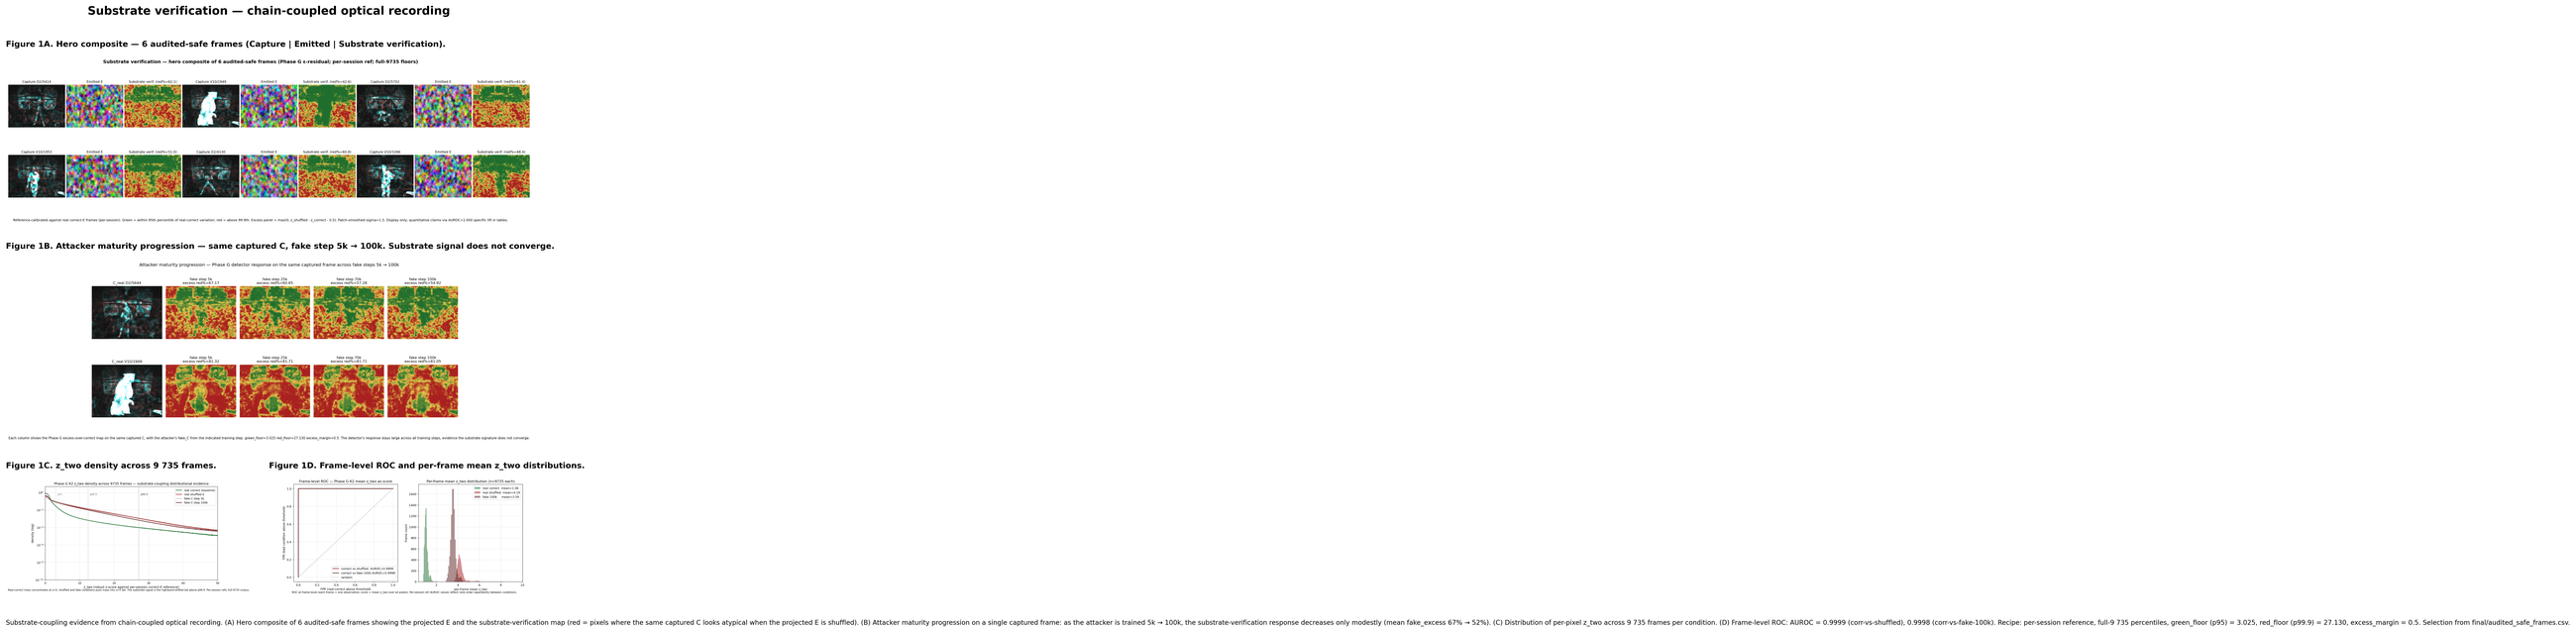
\includegraphics[width=\linewidth]{figures/fig_main_results.png}
\caption{Main result. (A)~Hero composite of substrate-verification maps for
genuine vs.\ substrate-altered captures. (B)~Attacker-maturity progression: the
same captured frame scored against synthetic emissions from adversary training
steps 5k--100k; the verification map stays strongly red at every maturity, i.e.\
the substrate signature does not converge as the attacker trains.
(C)~$z_{\text{two}}$ density across \num{9735} frames per condition.
(D)~Frame-level ROC and per-frame mean-$z$ distributions. Frame-level
AUROC~$=0.9999$ (correct vs.\ shuffled $E$) and AUROC~$=0.9998$ (correct vs.\
synthetic $E$ at step 100k) on this corpus. All maps use per-session references
and full-\num{9735} percentile floors with common thresholds within each paired
panel; AUROC values reflect rank-order separability between conditions on the
evaluated frame set, not a deployed operating point.}
\label{fig:main_results}
\end{figure}

\begin{figure}[t]
\centering
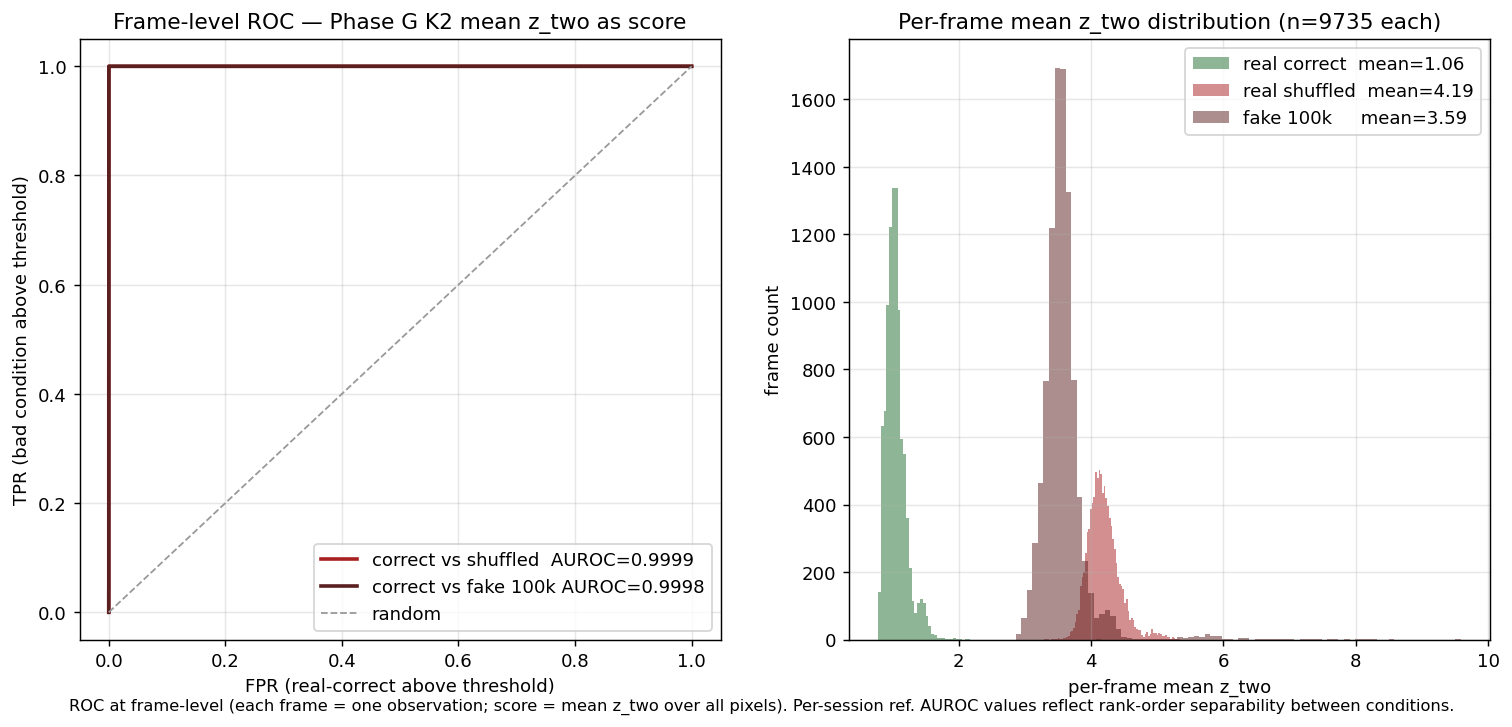
\includegraphics[width=\linewidth]{figures/fig_roc.png}
\caption{Frame-level separability. Left: ROC computed at the frame level, where
each frame is one observation and the score is the mean $z_{\text{two}}$ over all
pixels, giving AUROC = 0.9999 for correct vs.\ shuffled $E$ and AUROC = 0.9998
for correct vs.\ synthetic $E$ at training step \num{100000}. Right: per-frame
mean-$z_{\text{two}}$ distributions for the three conditions ($n=\num{9735}$
each), with the real-correct mode near $z=1.06$ and the shuffled ($4.19$) and
synthetic-\num{100000} ($3.59$) modes well separated from it. Per-session
reference; AUROC reflects rank-order separability between conditions on this
corpus, not a fixed-threshold field deployment.}
\label{fig:roc}
\end{figure}

\begin{figure}[t]
\centering
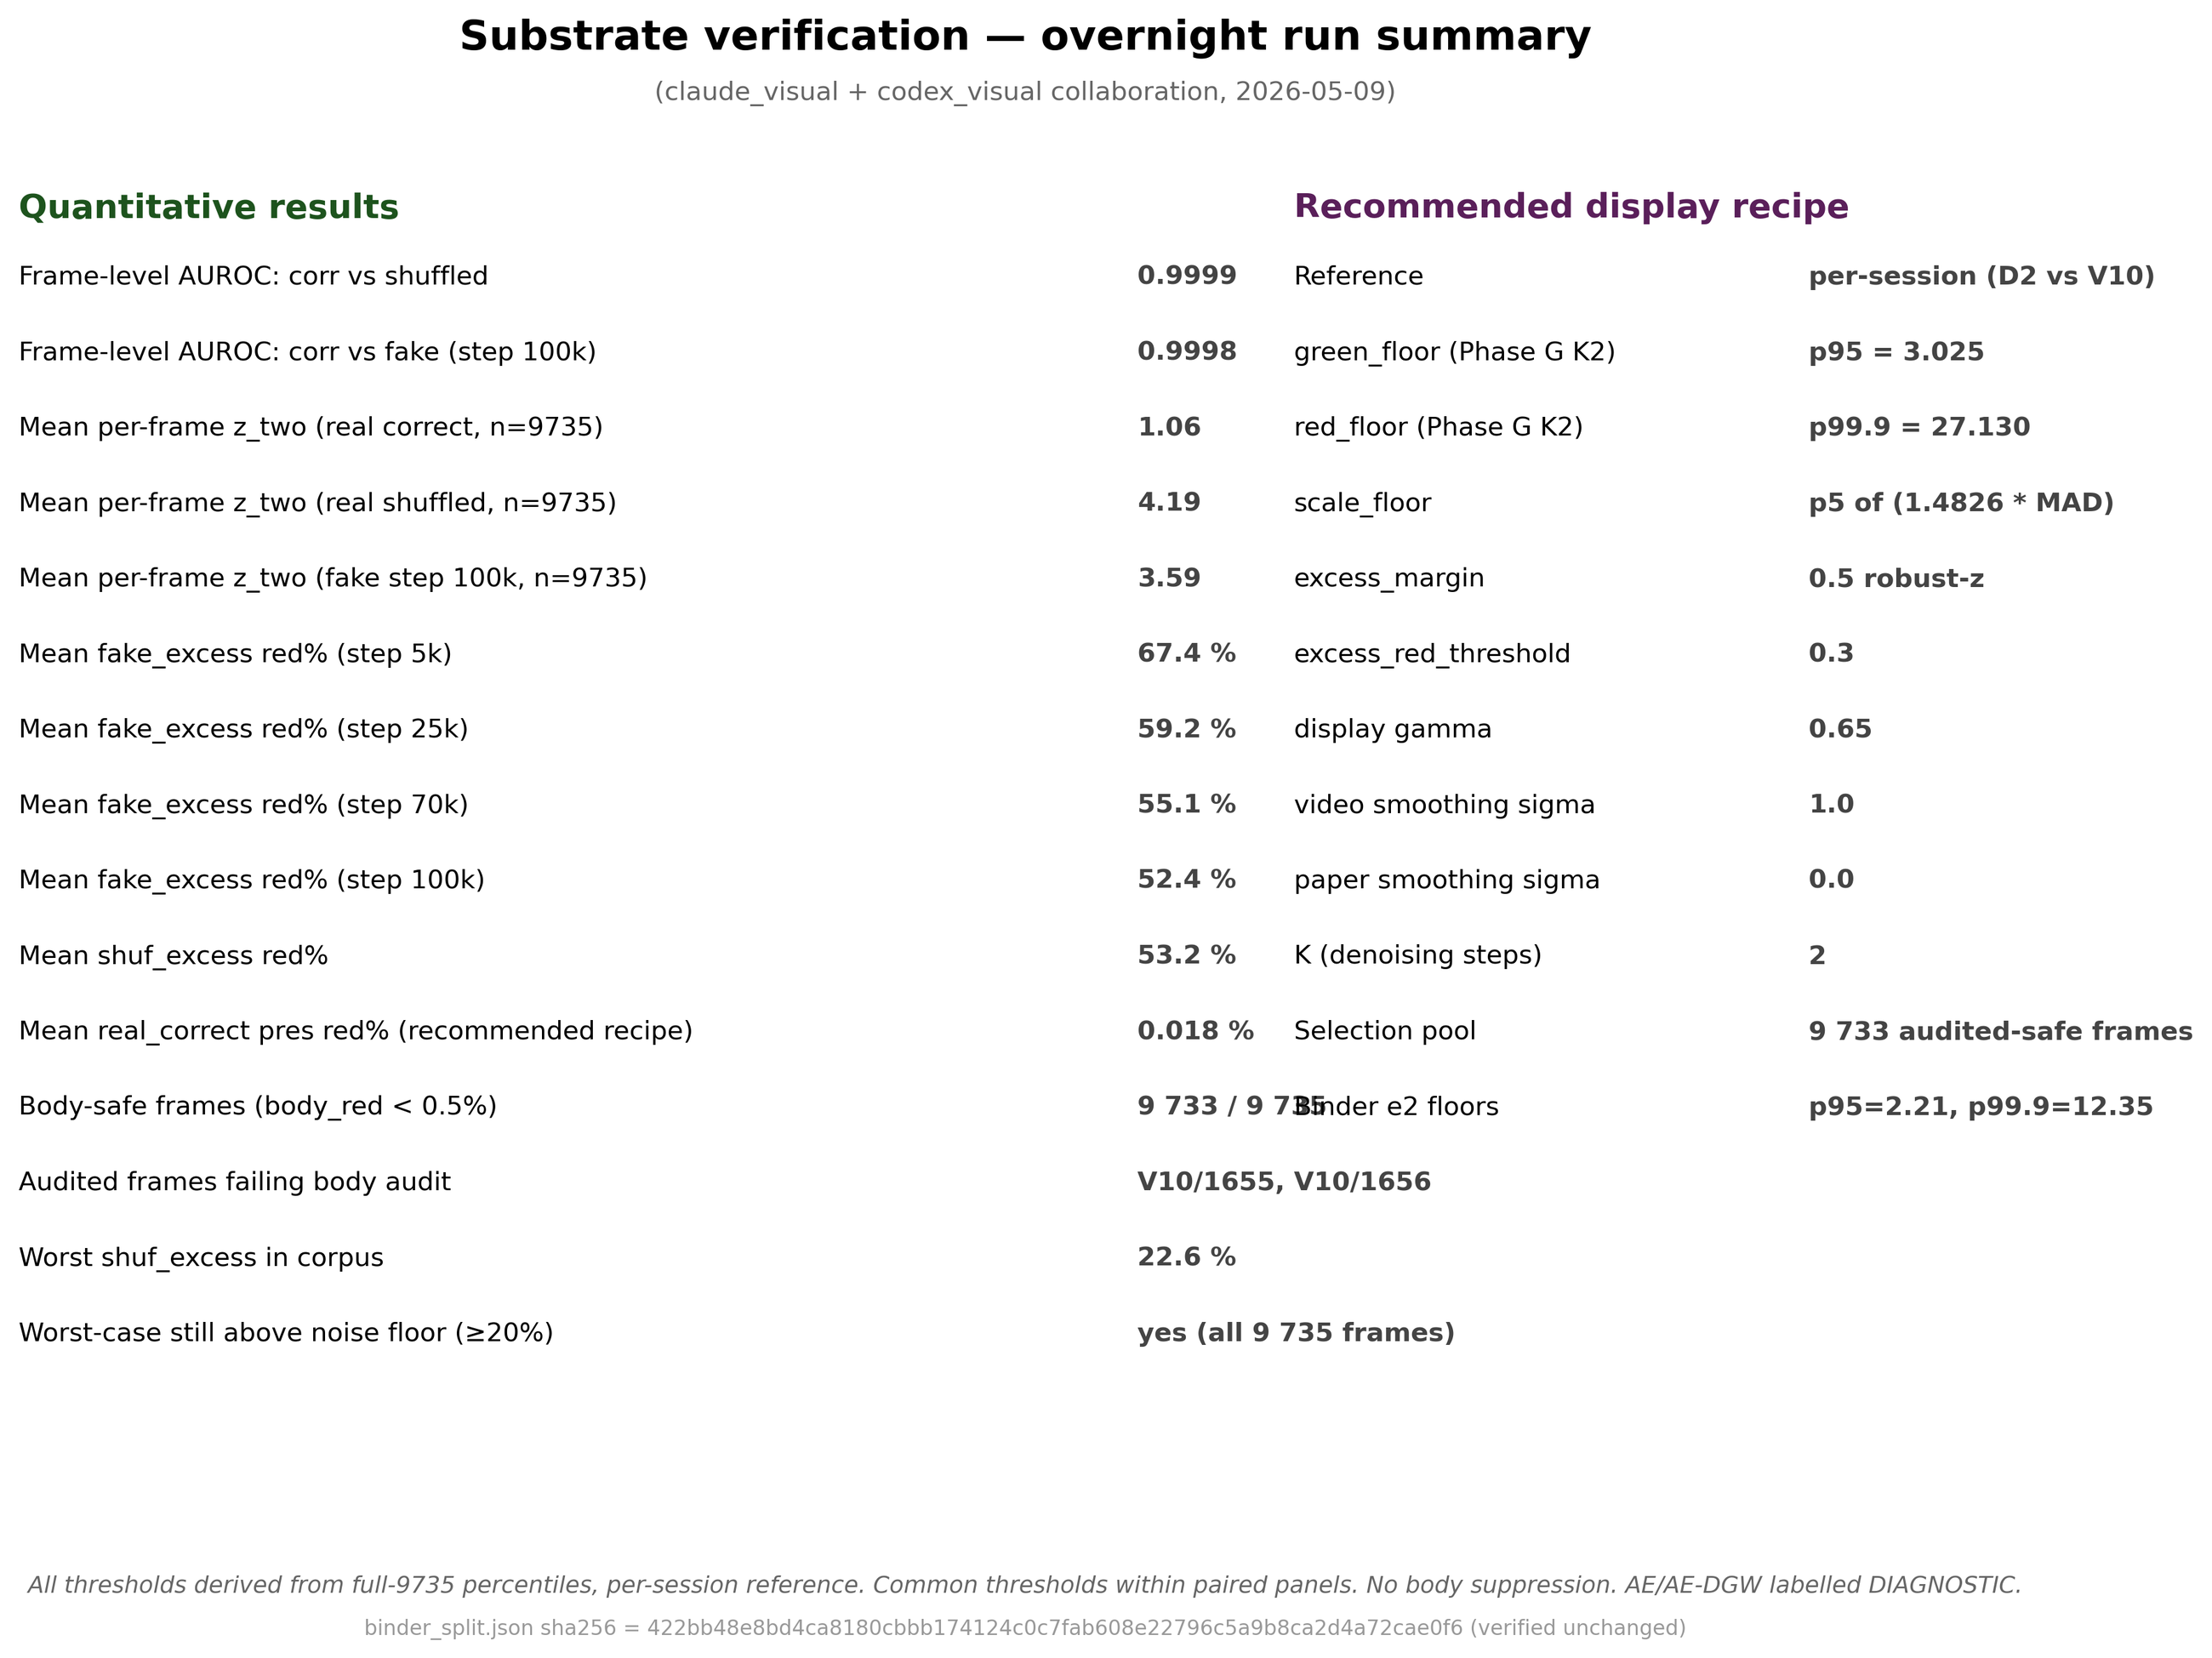
\includegraphics[width=\linewidth]{figures/fig_quant_table.png}
\caption{Quantitative summary and display recipe. Left: headline metrics ---
frame-level AUROC $0.9999$ (vs.\ shuffled) and $0.9998$ (vs.\ synthetic at step
\num{100000}); mean per-frame $z_{\text{two}}$ of $1.06$ (real-correct), $4.19$
(shuffled), $3.59$ (synthetic-\num{100000}); mean synthetic excess red\% declining
$67.4 \rightarrow 52.4$ across training steps \num{5000}\,$\rightarrow$\,\num{100000};
mean real-correct red\% $0.018\%$; \num{9733}/\num{9735} body-safe frames. Right:
the Phase~G K2 display recipe (green\_floor $=$ p95 $= 3.025$, red\_floor $=$ p99.9
$= 27.13$, scale\_floor $=$ p5 of $1.4826\cdot\mathrm{MAD}$, excess\_margin $0.5$,
$\gamma = 0.65$, $K=2$, per-session reference). All thresholds derived from
full-\num{9735} percentiles; common thresholds within paired panels; no body
suppression; AE/AE-DGW labeled DIAGNOSTIC.}
\label{fig:quant_table}
\end{figure}

\subsection{Same-rig cross-session and cross-protocol generalization}
\label{sec:results_main_generalization}

The main verifier is trained on real pairs from both sessions, so its held-out
blocks --- though strictly excluded from training with a \num{60}-frame guard
band and stride decimation --- are drawn from the same sessions seen in training.
To test whether the learned coupling transfers \emph{across} sessions, we run a
cross-session ablation: train the verifier on one session only and evaluate on
the entirely held-out other session. A D2-only verifier evaluated on held-out V10
achieves \textbf{AUROC = 1.0} for real-correct versus wrong/shuffled emissions,
and a V10-only verifier evaluated on held-out D2 likewise achieves
\textbf{AUROC = 1.0} (checkpoint step \num{100000}; both
$\text{real\_correct\_vs\_real\_shuffled} = 1.0$ and
$\text{real\_correct\_vs\_fake\_correct} = 1.0$). The verifier therefore does not
memorize a single session's emission statistics; the coupling it learns transfers
to a session it never saw during training.

This generalization is additionally cross-protocol. The two sessions were
recorded under structurally distinct chain transitions: D2 uses the v9 chain
(\texttt{ROW\_DOMAIN\_TAG} \texttt{b"TB:ROW:v9"}) and V10 uses the v10 chain
(\texttt{b"TB:ROW:v10"}), which additionally folds a \SI{32}{byte}
\texttt{ai\_payload\_root} committing AI-agent response frames into the state
transition $S_{t+1}$. A verifier trained on one protocol and evaluated on the
other still reaches AUROC = 1.0 on the real-correct-versus-wrong task, so the
result is a same-rig \emph{cross-protocol} generalization in addition to
cross-session. (Protocol version is confounded with session in this corpus ---
each protocol appears in exactly one session --- so we claim that verification
works across both versions, not that protocol version has no effect.)

\paragraph{Scope of the generalization claim.}
This result is strictly \emph{same-rig cross-session} (and same-rig
cross-protocol). It does \textbf{not} demonstrate cross-rig, cross-camera,
cross-projector, or cross-subject generalization; no such experiment exists in
this release, and whether the verifier generalizes beyond a single rig and a
single performer is untested. We are equally careful not to overstate uniformity within
the cross-session ablation. While the \emph{headline} real-correct-versus-shuffled
discrimination holds at AUROC = 1.0 out of distribution, other conditions degrade
when the verifier scores a session it was not trained on. The harder fake-pair
discrimination (fake\_correct vs.\ fake\_shuffled) drops out of distribution --- a
D2-only verifier on held-out V10 fakes falls to $0.8588$, versus $0.9295$ for the
combined verifier --- and the real-pair-versus-zero-$E$ AUROC also falls (e.g.\ a
D2-only verifier reaches $0.7221$ on V10). These drops indicate that part of the
verifier's coupling signal is session-specific. We therefore claim only that the
genuine-versus-anomalous separation transfers across same-rig sessions and
protocols; we do not claim uniform AUROC = 1.0 across all conditions, and we do
not claim robustness against the stronger F-A~v2 attacker, which is design-only
and not trained (see \Cref{sec:results_redteam}).

\subsection{Summary}
\label{sec:results_main_summary}

Three results anchor this section. First, the Phase~G verifier achieves
AUROC = 1.000 on held-out blocks of both sessions, with a tightly bounded
residual gap ($\Delta_{\text{wrong}} \approx +4\times10^{-3}$) that the
architecture- and data-matched shuffled control reduces to chance
(AUROC $\approx 0.5006$, $\Delta_{\text{wrong}} \approx 10^{-7}$), establishing
that the discrimination derives from genuine $C_t$--$E_t$ chain-coupling rather
than emission statistics or architecture. Second, at the frame level over the
full \num{9735}-frame corpus, the verifier reaches AUROC = 0.9999 against
shuffled emissions and AUROC = 0.9998 against F-A~v1 fakes at step \num{100000},
with real-correct frames rendering essentially green ($0.018\%$ mean red) and
anomalous conditions heavily red ($\sim$\,$51$--$53\%$). Third, the coupling
transfers same-rig across both sessions and both chain protocols at AUROC = 1.0
on the real-correct-versus-wrong task --- a generalization we bound explicitly to
same-rig scope, with documented out-of-distribution degradation on the harder
fake-pair and zero-$E$ conditions, and no claim beyond a single rig, two
sessions of one performer, and the single trained attacker F-A~v1.
